\chapter{Architecture and Design}

\section{Scenario Definition}
This project is considering a very specific scenario that involves the transportation of artwork from one place to another. More specifically a \textit{sender} is handing custody of the artwork to a \textit{carrier} who is responsible to transport the artwork safely to a \textit{receiver}. Upon arrival, the artwork's custody is transferred to the \textit{receiver}. During the transportation of the artwork environmental data like temperature and humidity is recorded and made available for monitoring purposes.

\begin{figure}
    \centering
    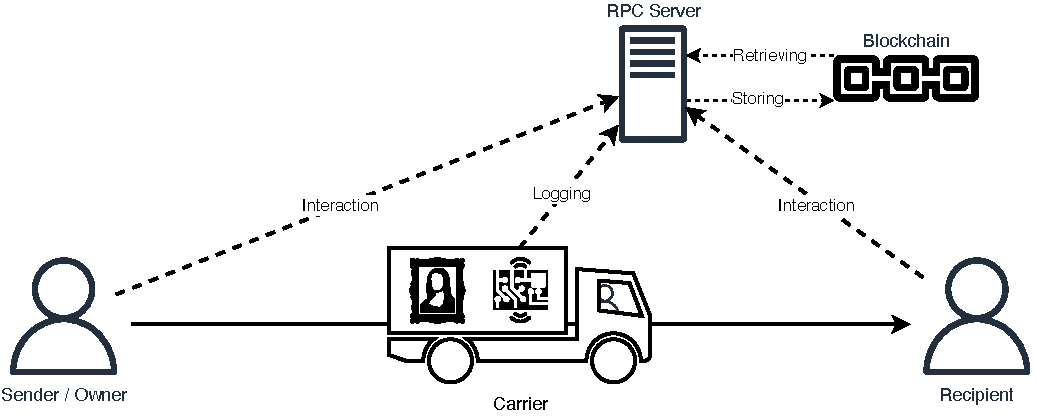
\includegraphics[width=0.8\textwidth]{diagrams/Scenario.drawio.pdf}
    \caption{Defined scenario for the system to consider}
    \label{fig:scenario}
\end{figure}

\subsection*{Summary of Abstractions}
The real-world scenario of transferring custody of artwork for transportation is naturally much more complex and involves more actors. \cite{artintransit} However in this work we are making the following abstractions:
\begin{itemize}
    \item The sender of a specific artwork is also the owner of the artwork
    \item When considering the transportation of the artwork back to the location of origin, the \textit{sender} and \textit{receiver} are the same.
    \item The authenticity and integrity of the artwork can be verified by any of the actors
\end{itemize}

\section{Overview}
Since the system is considering a very specific scenario This chapter aims to provide a high-level overview of the architecture of the system while later going into detail about its components and actors.

\subsection{Actors}

\begin{figure}
    \centering
    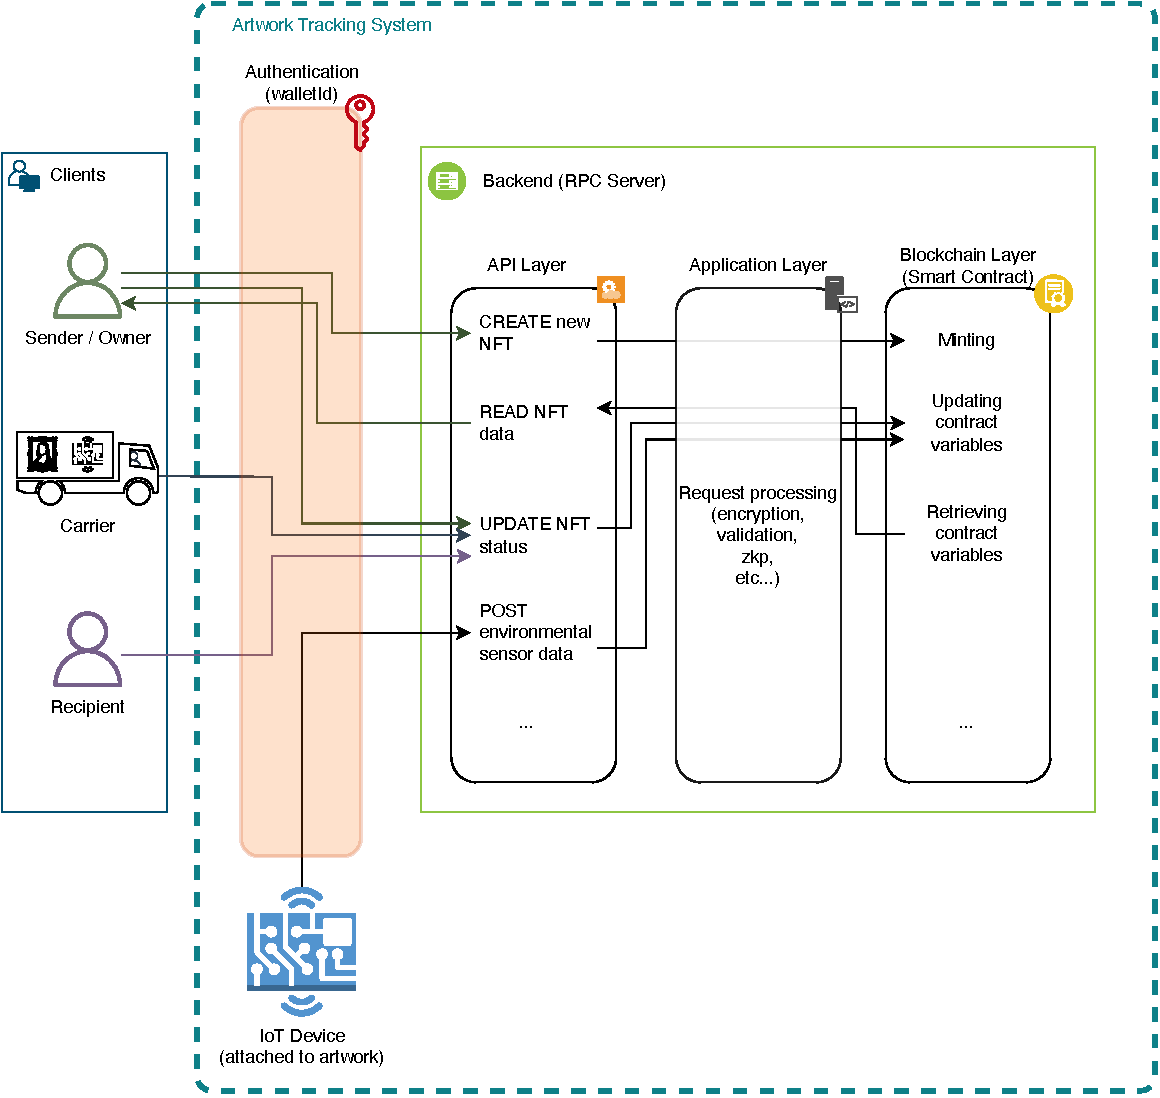
\includegraphics[width=\textwidth]{diagrams/Architecture.drawio.pdf}
    \caption{High-Level architecture design}
    \label{fig:architecture}
\end{figure}
